\chapter{数值模型的理论基础}
数值模拟已经成为内燃机设计开发和优化过程中的一个重要研究手段。由于内燃机工作过程中缸内形成高温和高压的环境
现有的测试方法很难直接将传感器安装在缸内进行测量,因此数值模拟在内燃机工作过程的研究上得到了广泛应用。
\section{离子电流模型}
点燃式内燃机在燃烧过程中,产生大量的化学反应,在缸内会产生大量的带电粒子\cite{ljwwty2008},并且这些带电粒子的运动具有无规律的特性。
如果在火花塞两级施加一个稳定的直偏电压,由于有外加电场存在,带电粒子发生定向迁移,从而形成了火花塞离子电流。\par
以下的离子电流模型是基于以下的几个假设而成立的:
\begin{itemize}
\item 火花塞间隙中的燃气完全燃烧
\item 燃烧过程满足绝热过程
\item 燃气满足热力学平衡
\item 火花塞间隙近似成圆柱模型
\end{itemize}
\subsection{缸内燃烧化学反应式}
通常认为离子电流主要产生在两个时期:火焰前锋期和火焰后期。点火开始后,火焰前锋面从火花塞点火处开始燃烧,此时形成离子电流的火焰
前锋期;当火焰前锋面离开火花塞两端时为离子电流的火焰后期\cite{ljw2004phd}。其中火焰前锋期的主要化学反应如下:
\begin{align}
CH+O\stackrel{K_{1}}{\longrightarrow}CHO^{+}+e^{-}\\
CHO^{+}+H_{2}O\stackrel{K_{2}}{\longrightarrow}H_{3}O^{+}+CO\\
CH+C_{2}H_{2}\stackrel{}{\longrightarrow}C_{3}H_{3}+e^{-}\\
H_{3}O^{+}+e^{-}\stackrel{K_{3}}{\longrightarrow}H_{2}O+H
\end{align}
其中$K_{i}(i=1,2,3)$表示反应常数,大小分别为:
\begin{align}
K_{1}=5\times10^{-14}cm^{3}/s\\
K_{2}=7\times10^{-9}cm^{3}/s\\
K_{3}=2.3\times10^{-9}cm^{3}/s
\end{align}
可以看到在火焰前锋期产生的主要离子是$H_{3}O^{+}$,这是在火焰前锋期产生离子电流的主要原因。
在后火焰期,不同于火焰前锋期中产生的大量$H_{3}O^{+}$,此时的$H_{3}O^{+}$离子已经基本上被消耗完了。
由于火焰前锋期产生的大量热导致缸内的温度较高,同时火焰在传播过程中火焰锋面直径越来越大,产生的热量增多,此时的离子电流以热电离为主。
研究表明\cite{reinmann1997local},$NO$的热电离产生了95\%的有效的自由电子,$NO$是火焰后区内产生电离过程的主要物质。$NO$起主导作用的原因
见表\ref{tab:nozx},可以看到其浓度在火焰后期中最大,且其电离率也是最大的。
\begin{table}[!h]
	\centering
	\caption{燃气中主要物质的电离参数}
	\label{tab:nozx}
	\begin{tabular}{|c|rl|c|c|}
		\hline
		物质			    &    \multicolumn{2}{c|}{电离能$/eV$}    &    浓度(在$15^{\circ} CA\ ATDC$时)    &    电离率\\\hline
		$NO$    		&   9.264&05     	&$1.48 \times 10^{-2}$  &  $2.44 \times 10^{-8}$\\\hline
		$H_{2}O_{2}$    &   10.540&00 		&$1.60 \times 10^{-6}$  & $1.73 \times 10^{-9}$\\\hline
		$CO$			&	14.013&90		&$4.85 \times 10^{-2}$	& $1.30 \times 10^{-12}$\\\hline
		$CO_{2}$		&	13.777&00		&$7.17 \times 10^{-2}$	& $2.10 \times 10^{-12}$\\\hline
		$H_{2}O$		&	12.618&80		&$1.16 \times 10^{-1}$	& $2.33 \times 10^{-11}$\\\hline
		$N_{2}$			&	15.580&80		&$6.99 \times 10^{-1}$	& $5.03 \times 10^{-14}$\\\hline
		$H_{2}$			&	15.425&89		&$9.72 \times 10^{-3}$	& $6.87 \times 10^{-14}$\\\hline
	\end{tabular}
\end{table}
根据Thermal或Zeldovich\cite{zeldovich1946oxidation}机理可以知道,$NO$主要是在1000摄氏度以上的高温情况下才会产生,这符合火焰后期的缸内温度情况。
其后火焰期的主要化学反应为:
\begin{align}
O+N_{2}\longleftrightarrow NO+N\\
N+O_{2}\longleftrightarrow NO+O\\
N+OH\longleftrightarrow NO+H
\end{align}
\par
由于$NO$是火焰后期产生离子电流的主要原因,因此$NO$浓度越高,离子电流越大。当$NO$达到最大值的时候,也即是燃烧最为充分的时候,此时对应最高缸压。因此火焰后期
的离子电流和缸内压力有很明确的关系。\par
总的来说,火焰前锋期的离子电流主要是化学电离产生的$H_{3}O^{+}$导致的;火焰后期的离子电流主要是$NO$热电离产生的电子导致的。
\subsection{火花塞离子电流的数学模型}
首先讨论离子电流火焰前锋期的数学模型。
根据火焰前锋期的化学反应方程式可以得到各反应物和生成物的生成率。下式是$H_{3}O^{+}$在反应过程中满足的公式
\begin{equation}
\frac{d[H_{3}O^{+}]}{dt}=k_{2}[CHO^{+}][H_{2}O]-k_{3}[H_{3}O^{+}][e]
\end{equation}
当上式右边为零时,即为燃起的化学反应达到了平衡状态。同理,其他的反应物和生成物也满足类似的公式。于是可以得到:
\begin{equation}
%	[H_{3}O^{+}]=\frac{k_{2}[CHO^{+}][H_{2}O]}{k_{3}[e]}\\
%	[CHO^{+}]=\frac{k_{1}[CH][O]}{k_{2}[H_{2}O]}
	[H_{3}O^{+}]=[e]=(\frac{k_{1}[CH][O]}{k_{3}})^{1/2}
\end{equation}
\par  由于汽油的成分复杂,而且燃烧具有不确定性,因此很难通过模型计算出$[CH]$和$[O]$的浓度,且其浓度主要由混合气的
空燃比所决定。因此火焰前锋期的离子电流很难得到理想的模型。
其次讨论火焰后期的离子电流模型。
根据缸内燃烧化学反应的分析可以得出,$NO$是火焰后期中产生离子电流的主要原因,因此火焰后期离子电流计算第一步为计算NO的浓度。
在已知$NO$浓度的情况下,利用沙哈方程可以求解热电离产生的$NO^{+}$浓度和自由电子的电离率,由此可以求解出离子电流的火焰后期离子电流数学模型。\par 
沙哈方程的公式如下:
	\begin{equation}
		\frac{\chi^{2}}{1-\chi^{2}}p=\frac{(2\pi m_{e})^{3/2}}{h^{3}}(\kappa T)^{5/2}exp(-\frac{E_{i}}{\kappa T})
	\end{equation}
其中:$m_{e}$为电子质量;$h$为普朗克质量;$\kappa$为波尔兹曼常数;$T$为气体的绝对温度;$E_{i}$为电离能;$p$为缸内压力;$\chi$为电离率。\par 
如果将火花塞间隙局部看成一个圆柱形的等离子体,那么有
\begin{equation}
	I_{on}=eN_{a}\chi \mu E\pi r^{2}
\end{equation}
其中$N_{a}$为离子浓度。
离子浓度满足公式
\begin{equation}
	\frac{dN_{a}}{dt}=6\times10^{16}T_{eq}^{-1/2}exp[-\frac{69090}{T_{eq}}](O_{2})_{eq}^{1/2}(N_{2})_{eq}
\end{equation}
于是可以得到火花塞离子电流公式为
\begin{equation}
	\label{eqn:ion_eqn}
	I_{on}=e^{3/2}N_{a}\pi r^{2}(\frac{\kappa}{2})^{1/4}\sqrt{\frac{3.2\times10^{-2}}{pm_{e}\overline{\lambda}}ET^{5/2}exp(-\frac{E_{i}}{\kappa T})}
\end{equation}
其中$p$为缸内压力;$E$为外加电场强度;$r$为火花塞中心电极半径;$\overline{\lambda}$为电子平均自由程;$T$为气体的绝对温度;$E_{i}$为电离能;$m_{e}$为电子质量;
$\kappa$为波尔兹曼常数。
\section{电路结构与采集信号}
\subsection{电容式离子电流电路结构}
如下图\ref{fig:ionstruct}所示的是电容式离子电流检测电路结构。
\begin{figure}[!h]
	\centering
	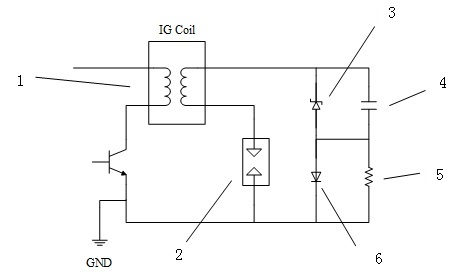
\includegraphics[width=0.8\textwidth]{thesis_figure/ion_struct}
	\caption{电容式离子电流检测电路结构}
	\label{fig:ionstruct}
\end{figure}
其中
\begin{enumerate}[1]
\item 表示点火线圈
\item 表示火花塞电极两段
\item 表示瞬态抑制二极管,防止电压过高使电路失效
\item 是电容,作为次级电路电源
\item 是检测电阻
\item 是普通二极管,用于限定检测电阻两端最大电压
\end{enumerate}
\subsection{电容式离子电流采集信号}
电容式离子电流分为三个时期:点火干扰期,火焰前锋期和火焰后期。如下图\ref{fig:ion_basic}所示是离子电流的三个时期\cite{saitzkoff1997cylinder}。
\begin{figure}[!h]
	\centering
	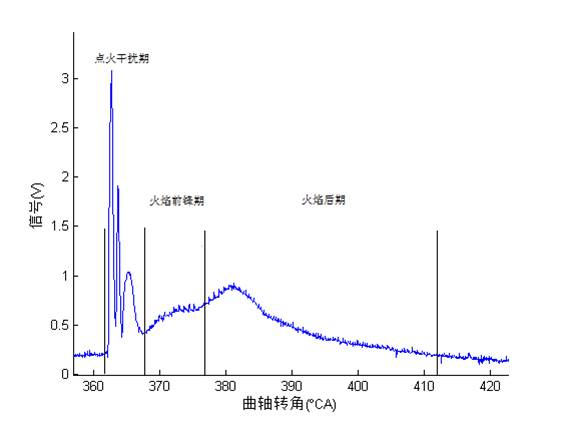
\includegraphics[width = 0.85\textwidth]{thesis_figure/model_chapter/ion_basic}
	\caption{电容式离子电流的三个时期\cite{bh2007}}
	\label{fig:ion_basic}
\end{figure}
其中点火干扰期是由点火干扰造成的。火焰前锋期由火焰锋面经过电极附近的化学电离导致的;火焰后期由火焰锋面离开电极附近后的$NO$的热电离导致的。由于点火干扰的持续时间
和点火线圈的内部结构有关系,而火焰前锋期和火焰后期和燃烧有关系,所以点火干扰期可能会和火焰前锋期甚至是火焰后期相重合。但是点火干扰的曲线和火焰前锋或火焰后期的区别在于,点火干扰
期的曲线存在稳定的震荡信号,而化学电离或热电离导致的电流频率较低。通常来说火焰后期持续到整个燃烧阶段结束。
\section{小波分析}
\subsection{小波分析理论基础}
传统的信号分析手段主要是傅里叶变换,最早来自于傅里叶于1822年发表的热传导解析理论,从那时起傅里叶变换就成为了信号处理中的主要手段。傅里叶变换的
主要思想是将时域中的信息转换为频域中的信息,通过对频域中的信息进行处理从而达到了信号处理的目的。也正因为其本质是频域信息处理,且由于频域窗口容易
产生边界效应,傅里叶变换不能够完美的解决信号处理问题。1946年Gabor提出了著名的Gabor变换,随之发展成为了短时傅里叶变换,其本质仍然是一种加窗的傅里
叶变换,随后的几十年的信号处理领域,提出了多种不同的窗口都为了克服窗口的边界效应,但是都不能够从本质上解决信号处理的问题,只能够在低频信号中采用
大时间窗,高频信号中采用小时间窗的手段不完美的解决问题。\par
自从20世纪80年代末小波分析方法提出后,揭示了频域信号和时域信号之间关系的本质,提出了著名的影响深远的小波变换。
傅里叶变换是基于正弦信号的变换,而小波变换是基于小波函数的变换,因此傅里叶变换其实是小波变换的一种特例。由于小波基函数的正交性等特点,可以在信号的低频部分有较高的频率分辨率和较低
的时间分辨率,而在高频部分具有较高的时间分辨率和较低的频率分辨率\cite{lph2011},比傅里叶变换灵活多变,是傅里叶变换的数学本质上的前进。
\par 在实际应用中,计算机只能够处理离散化的信息,因此主要采用离散小波基函数进行小波分析。以下即是连续小波序列$\psi_{a,b}(t)$和连续小波变换$W_{f}(a,b)$的离散化。
在连续小波中,考虑小波函数
\begin{equation}
	\psi_{a,b}=|a|^{-\frac{1}{2}}\psi(\frac{t-b}{a})
\end{equation}
这里$b\in R$,$a\in R_{+}$,且$a\neq0$,$\phi$是容许的,为方便起见,在离散化中,总限制$a$只取正值,这样相容性条件\cite{lyhsz2008,dys2005}就变为
\begin{equation}
	C_{\psi}=\int^{\infty}_{0}\frac{\mid \widehat{\psi}(\overline{\omega})\mid}{\mid \overline{\omega}\mid}d\overline{\omega} < \infty
\end{equation}
通常\cite{shr2009},把连续小波变换中尺度参数$a$和平移参数$b$的离散化公式分别取作$a=a_{0}^{j}$,$b=ka_{0}^{j}b_{0}$,这里$j\in Z$,扩展步长$a_{0}\neq 1$是固定值,
通常来说,总是假定$a_{0}>1$,由于$m$可以取正也可以取负,因此假定不会影响结果。所以对应的离散小波变换函数$\psi_{j,k}(t)$即可写作
\begin{equation}
	\psi_{j,k}(t)=a^{-\frac{j}{2}}_{0}\psi(\frac{t-ka_{0}^{j}b0}{a_{0}^{j}})=a_{0}^{-\frac{j}{2}}\psi(a_{0}^{-\frac{j}{2}}t-kb_{0})
\end{equation}
而离散化小波系数则可表示为
\begin{equation}
	C_{j,k}=\int_{-\infty}^{\infty}f(t)\psi_{j,k}^{*}(t)dt=<f,\psi_{j,k}>
\end{equation}
其重构公式为
\begin{equation}
	f(t)=C\sum_{-\infty}^{\infty}\sum_{-\infty}^{\infty}C_{j,k}\psi_{j,k}(t)
\end{equation}
其中$C$是一个与信号无关的常数。由此可以看到信号序列$f(t)$可以由信号无关量$C$和小波函数$\psi$组成。
\subsection{多分辨率分析}
多分辨率分析是一种分析方法,其本质作用是可以得到构造小波函数和尺度函数的双尺度方程。通过这种方法,即使在不知道小波函数和尺度函数的解析公式的情况下,仍然可以
得到离散化的小波函数和尺度函数,从而可以解决离散化的小波分析问题。
\par 设$(\{ V_{m};m\in Z\} ;\phi(t))$是一个正交多分辨率分析,则存在$\{ h_{k} \}\in l^{2}$使得下面的双尺度方程
\begin{equation}
	\phi(x) = \sum_{k}h_{k}\phi(2x-k)
\end{equation}
成立,并且利用尺度函数$\phi(x)$构造小波函数
\begin{equation}
	\psi(x)=\sum_{ki}g_{k}\phi(2x-k)
\end{equation}
其中$h_{k}=2\int_{-\infty}^{\infty}\phi(x)\overline{\phi(2x-k)}dx$,$g_{k}=(-1)^{k}\overline{h_{1-k}}$。
\par 根据上述理论多分辨率分析可以得到离散化的尺度函数和小波函数的获得方法。
\subsection{小波函数分析步骤}
小波函数分析一共分为四步\cite{2006matlab}。第一步是采样。如果待分解的是模拟信号$f(t)$,选择$N=2^{n}$,得到采样信号值$a_{k}^{n}=f(\frac{k}{2^{n}})$,其中$k$的取值保证$\frac{k}{N}$位于信号$f(t)$发生的时间范围
之内,并在每个不小于$\frac{1}{N}$的时间段内都能取到采样信号$a_{k}^{n}=f(\frac{k}{2^{n}})$,于是可以用信号
\begin{gather}
f_{n}(x)=\sum_{k\in Z}a_{k}^{n}\phi(2^{n}x-k)
\end{gather}
对连续信号$f(t)$进行高精度的近似。
\par 第二步是分解。设信号$f_{n}(x)$逐级分解为
\begin{gather}
	f_{n}(x)=W_{n-1}(x)+W_{n-2}(x)+...+W_{l-1}(x)+f_{l-1}(x) \nonumber \\
			=W_{n-1}(x)+W_{n-2}(x)+...+W_{0}(x)+f_{0}(x)
\end{gather}
\par 其中
\begin{gather*}
W_{l-1}(x)=\sum_{k\in Z}b_{k}^{l-1}\psi(2^{l-1}x-k)\\
f_{l-1}(x)=\sum_{k\in Z}a_{k}^{l-1}\psi(2^{l-1}x-k)
\end{gather*}
系数$a_{k}^{l-1}$与$b_{k}^{l-1}$按照上标
从大到小的顺序从$l=n$开始直到$l=0$结束,满足
\begin{gather}
	b_{k}^{l-1}=\frac{a_{2k}^{l}-a_{2k+1}^{l}}{2}\\
	a_{k}^{l-1}=\frac{a_{2k}^{l}+a_{2k+1}^{l}}{2}
\end{gather}
\par 第三步是信号处理。将分解后的信号表示成下面的形式
\begin{gather}
	f_{n}(x)=\sum_{l=0}^{n-1}W_{l}(x)+f_{0}(x)\nonumber \\
			=\sum_{l=0}^{n-1}(\sum_{k\in Z}b_{k}^{l}\psi(2^{l}x-k))+\sum_{k\in Z}a_{k}^{0}\phi(x-k)
\end{gather}
信号处理的过程就是根据实际情况对$b_{k}^{l}$作适当的修正。
\par 第四步是信号重构。设重构后的信号值满足
\begin{equation}
	\widetilde{f_{n}}(x)=\sum_{k\in Z}a_{k}^{n}\phi(2^{n}x-k)
\end{equation}
则上述信号值可以通过下面的递推过程得到
\begin{equation}
	\widetilde{a}^{l}=\widetilde{L}U\widetilde{a}^{l-1}+\widetilde{H}U\widetilde{b}^{l-1}, l=1,2,3,...,n
\end{equation}
其中$\widetilde{a}^{l}$和$\widetilde{b}^{l}$,$l=0,1,2,3,...,n$是根据第二、第三步得到的修正系数。\par
在所有的四步计算中,最为主要的就是第三步信号处理过程,在该过程中对小波基函数的系数进行修正就可以得到不同的结果。如
果要对信号进行去噪,则可以对高频的小波基函数的系数进行清除;如果要对信号进行压缩处理,则可以对小波基函数的系数进行阈值设
定,从而去除不必要的频率的小波基函数。
\subsection{小波分析的特点}
\begin{enumerate}[1)]
	\item~\textbf{灵活性}\quad 由于小波基函数$\phi(x)$不是唯一的,通过小波函数的构造方法就可以构造出任意的小波基函数。
	但是小波基函数的构造要和问题相结合。而傅里叶变换不能够改变其变换的基函数,灵活性受到了很大的限制。
	\item~\textbf{快速性}\quad 由尺度函数和两尺度关系来推导的小波系数,在未知小波函数的解析表达式情况下也可以对信号进行分析。
	并且在不同的频率段上可以进行细分,而傅里叶分析无法做到对特定的频率段进行细分观察。
	\item~\textbf{双域性}\quad 小波分析是时频分析,同时揭示了频域和时域两个领域的信号特征。而傅里叶变换只能在单域中显示信号特性。
	\item~\textbf{深刻性}\quad 小波理论具有很深刻的数学根基,其发展来自于数学的推导而不是像傅里叶变换更多的来自于工程应用中。
\end{enumerate}
\subsection{常见的可离散小波}
常见的可离散小波主要有db小波,sym小波,coif小波和dmey小波。其中sym小波和coif小波都是db小波的改进版本,且db小波和sym小波都有阶数选择问题。这两个
小波的阶数越大,分析得到的信号越加的平滑。不仅如此,sym小波相对于db小波具有更好的对称性,因此在信号重构方面更加的不容易失真。coif小波具有最大为五阶
的阶数,其相对于db和sym小波来说具有更好的近似对称性。由于其最高只有五次阶数且是更近似对称小波,往往比db和sym小波有更快速的计算能力。
dmey小波是离散meyer小波,由于是标准的对称小波,有快速算法,往往比前面的几个小波计算速度更快。
\subsection{离散小波之间的比较}
根据不同的应用情况,需要选取不同的小波基函数,一般的选择原则如下:
\par (1)正交性。正交性的目的在于简化工程分析,方便对数据进行处理。
\par (2)紧支性。紧支性的小波具有很好的时频局部特性,能够比较方便的用计算机语言实现。
\par (3)对称性。对称的小波基函数具有线性相位特性,这种特性有利于对图像进行分析和重构,其重构图像的边缘不容易失真。
\par (4)正则性。正则性的小波基函数对信号分析之后产生的曲线平滑,是函数频域能量的一种度量。
\par (5)消失矩。消失矩的阶数越大,越是能够对信号的高频部分进行精细分析,同时可以提高信号的衰减程度。\par
下表\ref{tab:lsxb}所示的是所有的可以进行离散小波变换的小波比较\cite{wxf2003}。\par
\begin{table}[!h]
	\centering
	\caption{可离散变换的小波函数比较}
	\label{tab:lsxb}
	\begin{tabular}{|c|c|c|c|c|}
	\hline
	小波名称&正交性&双正交性&紧支撑性&支撑长度\\\hline
	db&是&是&是&2N-1\\\hline
	sym&是&是&是&2N-1\\\hline
	dmey&是&是&是&有限长度\\\hline
	coif&是&是&是&6N-1\\\hline
	\multicolumn{5}{c}{}
	\end{tabular}
	\begin{tabular}{|c|c|c|c|c|}
	\hline
	小波名称&滤波器长度&对称性&小波函数消失矩阶数&尺度函数消失矩阵数\\\hline
	db&2N&对称&N&-\\\hline
	sym&2N&近似对称&N&-\\\hline
	dmey&[-8,8]&对称&-&-\\\hline
	coif&6N&近似对称&2N&2N-1\\\hline
	\end{tabular}
\end{table}
小波类型的选择需要针对不同的问题采取不同的处理方式。
例如对于分段多项式结构组成的信号,db小波比较适用;局部三角函数基比较合适\cite{zyclz2004}分析包含正弦分量的信号。如何
根据分析信号的特点,结合任务来优化设计小波函数一直是值得探讨的问题,迄今为止还没有系统完整的总结。且对于一些特定的离散问题,还可以通过利用多分辨率分析的方法自己构造离散的尺度函数和
小波函数。
\section{高斯曲线拟合}
\subsection{高斯函数}
高斯函数是在各个学科和工程中广泛使用的一种函数。高斯函数的形式为:
\begin{equation}
	f(x)=ae^{-\frac{(x-b)^2}{c^2}}
\end{equation}
其中$a$,$b$,$c$为实常数,且$a>0$。
\par  $c^2=2$的高斯函数是傅里叶变换的特征函数\cite{wcpyh2006}。对高斯函数进行傅里叶变化不会改变函数的本质,仍然是高斯函数。
高斯函数的不定积分是误差函数。\par
\subsection{离子电流拟合原理和方法}
Saitzkoff\cite{saitzkoff1996ionization}在缸内气体完全燃烧并且达到热化学平衡情况下推导了火焰后期的离子电流的理论公式。
\begin{equation}
	\frac{I}{I_{m}}=\frac{1}{\frac{p}{p_m}}^{\frac{1}{2}-\frac{3}{4}\frac{\gamma -1}{\gamma}}e^{-\frac{E_i}{2\kappa T_m}[\frac{1}{(\frac{p}{p_m})^{\frac{\gamma -1}{\gamma}}}-1]}
\end{equation}
其中$I$是离子电流,$I_{m}$是离子电流最大值,$p$是缸压,$p_{m}$是缸压最大值,$T_{m}$是缸内最大温度,$\gamma$是比热容比,$\kappa$是波尔兹曼常数,$E_{i}$是
离子电流能量。该公式与高斯函数相近。所以可以将火焰后期的离子电流近似拟合成高斯曲线。\par
L.Eriksson和L.Nielsen\cite{eriksson1996ignition,eriksson1997closed,eriksson1997ionization}采用该方法能够准确地估计缸压最值对应相位,从而可以
自适应调整点火提前角,提高了发动机的燃烧效率。Magnus Hellring等人也通过了拟合曲线的方法控制了缸压峰值相位的位置\cite{hellring2001comparison}。\par
而由于排气过程不能将缸内的所有废气排除缸内,断油循环和断火循环中仍然存在部分带$NO$离子
的废气,仍然可以检测到离子电流。同样道理,在正常循环的点火之前由于存在部分废气,离子电流检测电路可以检测到轻微的离子电流信号。这部分废气导致的离子电流信号也可以用高斯函数近似分析。
由此整个检测到的离子电流信号可以用两个高斯曲线拟合来进行分析。





